\documentclass[leqno]{article}
\usepackage{graphicx} % Required for inserting images
\usepackage[top=0.9in, bottom=1in, left=1.5in, right=1.5in]{geometry}
\usepackage[utf8]{inputenc}
\usepackage[icelandic]{babel}
\usepackage[T1]{fontenc}
\usepackage[parfill]{parskip}
% Tables and lists
\usepackage{booktabs,tabularx}
\usepackage{multirow}
\usepackage{enumerate}
\usepackage{adjustbox}
\usepackage{multicol}
\usepackage{xcolor}
\usepackage{algpseudocode}
\usepackage{tikz}
\usepackage{listings}
\lstset{
	basicstyle=\ttfamily,
	mathescape
}
\usetikzlibrary{arrows, positioning, calc, graphs}
\tikzset{
node distance=5mm,
>=stealth',
black!70,
text=black,
graphs/every graph/.style={edges=rounded corners},
vloop/.style={to path={-- ++(#1,0) |- (\tikztotarget)}},
hloop/.style={to path={-- ++($(0,0)-(#1,0)$) |- (\tikztotarget)}},
downright/.style={to path={-- ++(0.7,0) |- (\tikztotarget)}},
rightup/.style={to path={-- ++(1,0) |- (\tikztotarget)}},
hv path/.style={to path={-| (\tikztotarget)}},
vh path/.style={to path={|- (\tikztotarget)}},
box/.style={%
    rectangle,
    minimum size=6mm,
	rounded corners=1mm,
    draw=black,
    % Font
    %font=\itshape
},
start/.style={%
    circle,inner sep=1pt,minimum size=1pt,fill=white,draw=black!70,text=black!70
},
end/.style={%
    start, draw=black,text=black,
},
junction/.style={circle,inner sep=0pt,minimum size=0pt},
}


% Math
\usepackage{amsmath, amssymb}
% Graphics

\usepackage{graphicx}
% Code environment
\usepackage{minted}

\renewcommand\thesubsection{}

\title{Forritunarmál Hópverkefni 1}
\author{Ragnar Björn Ingvarsson, rbi3, \\ 
Daníel Snær Halldórsson, dsh11, \\
}

\begin{document}
	
	\maketitle

	\newpage
	\section{Hvað er mál?}

	Svarið hér er \textbf{(B)}, Mengi strengja.

	\section{Sýnið BNF, EBNF og málrit fyrir eftirfarandi mál}

	\subsection{a) $\{a^nb^kc^n|n,k \in \mathbb{N}\}$}

		\begin{center}\begin{tabular}{rl}
				\textbf{BNF:} &
			\begin{lstlisting}
<R> ::= a <R> c | <B>
			\end{lstlisting} \\
							  & \begin{lstlisting}
<B> ::= b <B> | $\lambda$ 
			  \end{lstlisting} \\[5ex]

				\textbf{EBNF:} &
			\begin{lstlisting}
R = 'a', R, 'c' | {'b'};
			\end{lstlisting} \\[5ex]
				\textbf{Málrit:} &
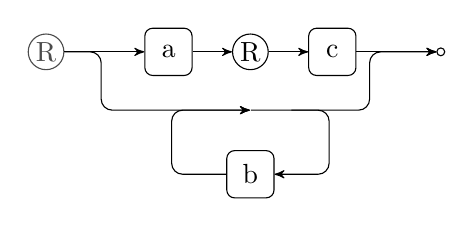
\begin{tikzpicture}

\node[start] (start) {R};
\node[junction,right=of start] (p1) {};
\node[box,right=of p1] (a) {a};
\node[end,right=of a] (R) {R};
\node[box,right=of R] (c) {c};
\node[junction,below=of R] (b) {};
\node[junction,right=of c] (p2) {};
\node[end,right=of p2] (end) {};
\node[junction,left=of b] (p3) {};
\node[box,below=of b] (p4) {b};
\node[junction,right=of b] (p5) {};

\graph [use existing nodes] {
start -> a -> R -> c -> end;
start ->[downright] b;
p5 ->[rightup] end;
b ->[vloop] p4;
p4 ->[hloop] b;
};

\end{tikzpicture} \\


		\end{tabular}
	\end{center}

		\subsection{b) $\{(ab)^nc^kd^k|n,k \in \mathbb{N}\}$}

		\begin{center}\begin{tabular}[t]{rl}
				\textbf{BNF:} &
			\begin{lstlisting}
<R> ::= <abpart> <cdpart>
			\end{lstlisting} \\
							  & \begin{lstlisting}
<abpart> ::= ab <abpart> | $\lambda$
			\end{lstlisting} \\
							  & \begin{lstlisting}
<cdpart> ::= c <cdpart> d | $\lambda$
			\end{lstlisting} \\[5ex]

				\textbf{EBNF:} &
			\begin{lstlisting}
R = {'ab'}, cdpart;
			\end{lstlisting} \\
							  & \begin{lstlisting}
cdpart = ['c', cdpart, 'd'];
			\end{lstlisting} \\[8ex]

				\textbf{Málrit:} &

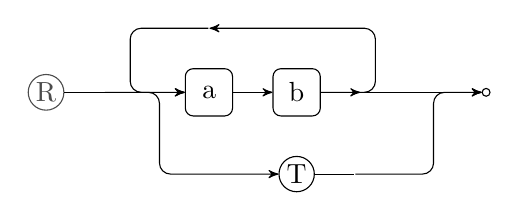
\begin{tikzpicture}
	\node[start, text=black!70] (start) {R};
	\node[junction, right=of start] (p1) {};
	\node[junction, right=of p1] (p2) {};
	\node[box, right=of p2] (a) {a};
	\node[box, right=of a] (b) {b};
	\node[junction, right=of b] (p3) {};
	\node[junction, right=of p3] (p4) {};
	\node[junction, right=of p4] (p6) {};
	\node[end, right=of p6] (end) {};
	\node[end, below=of b] (cdpart) {T};
	\node[junction, above=of a] (p5) {};
	\node[junction, right=of cdpart] (p7) {};


\graph [use existing nodes] {
start -> a -> b -> p3 -> end;
p1 ->[downright] cdpart;
cdpart -- p7 ->[rightup] end;
b ->[vloop] p5;
p5 ->[hloop] a;
};

\end{tikzpicture} \\ \\
& 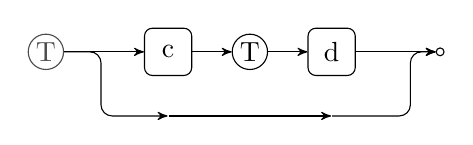
\begin{tikzpicture}
	\node[start, text=black!70] (start) {T};
	\node[junction, right=of start] (p1) {};
	\node[box, right=of p1] (c) {c};
	\node[end, right=of c] (T) {T};
	\node[box, right=of T] (d) {d};
	\node[junction, right=of d] (p2) {};
	\node[end, right=of p2] (end) {};
	\node[junction, below=of c] (p3) {};
	\node[junction, below=of d] (p4) {};

\graph [use existing nodes] {
start -> c -> T -> d -> end;
start ->[downright] p3;
p3 -> p4;
p4 ->[rightup] end;
};
\end{tikzpicture}

			\end{tabular}
		\end{center}

	\subsection{c) $\{a^nb^nc^n|n \in \mathbb{N}\}$}

			Það er ekki hægt að setja þetta á BNF þar sem 
			ómögulegt er að bæta við þriðja tákninu því ekki er 
			hægt að staðfesta að það birtist nákvæmlega $n$ sinnum.

			Aðferðin sem við höfum notað til að fá $a^nb^n$ hingað til 
			felst í því setja $a$ og $b$ hvoru megin við endurkvæmnina 
			en ekki er hægt að gera það með þremur stökum.

			Einnig kemst þetta ekki á EBNF og heldur ekki sem málrit því 
			hvort tveggja fylgir sömu grunnvirkni og BNF.

		\subsection{d) $\{a^nb^nc^k|n,k \in \mathbb{N}\}$}

		\begin{center}\begin{tabular}{rl}
				\textbf{BNF:} &
			\begin{lstlisting}
<R> ::= <abpart> <cpart>
			\end{lstlisting} \\
							  & \begin{lstlisting}
<abpart> ::= a <abpart> b | $\lambda$
			\end{lstlisting} \\
							  & \begin{lstlisting}
<cpart> ::= c <cpart> | $\lambda$
							  \end{lstlisting} \\[5ex]

				\textbf{EBNF:} &
			\begin{lstlisting}
R = abpart, {'c'};
			\end{lstlisting} \\
							  & \begin{lstlisting}
abpart = ['a', abpart, 'b'];
							  \end{lstlisting} \\[5ex]

				\textbf{Málrit:} & 
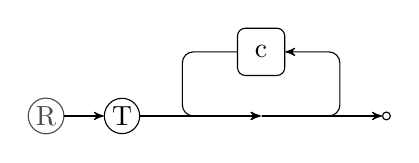
\begin{tikzpicture}
	\node[start] (start) {R};
	\node[end, right=of start] (T) {T};
	\node[junction, right=of T] (p) {};
	\node[junction, right=of p] (p1) {};
	\node[junction, right=of p1] (c) {};
	\node[junction, right=of c] (p2) {};
	\node[box, above=of c] (p3) {c};
	\node[junction, right=of p2] (p4) {};
	\node[end, right=of p4] (end) {};

\graph [use existing nodes] {
start -> T -> c -> end;
c ->[vloop] p3;
p3 ->[hloop] c;
};
\end{tikzpicture} \\ \\
& 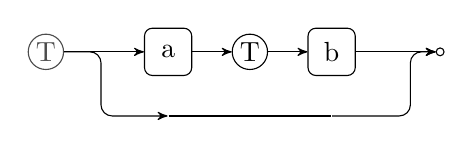
\begin{tikzpicture}
	\node[start] (start) {T};
	\node[junction, right=of start] (p1) {};
	\node[box, right=of p1] (a) {a};
	\node[end, right=of a] (T) {T};
	\node[box, right=of T] (b) {b};
	\node[junction, right=of b] (p2) {};
	\node[junction, below=of a] (p3) {};
	\node[junction, below=of b] (p4) {};
	\node[end, right=of p2] (end) {};

\graph [use existing nodes] {
start -> a -> T -> b -> end;
start ->[downright] p3 -- p4 ->[rightup] end;
};
\end{tikzpicture} \\[5ex]
			\end{tabular}
		\end{center}


		\section{Lýsið því máli sem BNF-mállýsingin skilgreinir}
		\[
			\langle x \rangle ::= x  \langle x \rangle
		\]\[
		\hspace{1em} | \hspace{1em} \langle y \rangle
		\]
		\[
			\langle y \rangle ::= y  \langle y \rangle
		\]\[
		\hspace{.2em} | \hspace{1em} \lambda
		\]


		Við sjáum að BNF-mállýsingin myndi vera skrifuð sem $x^*y^*$ með 
		reglulegri segð og við getum þá lýst málinu sem óákveðið mörg x, 
		fylgd eftir af óákveðið mörgum y.

		Málrit væri þá svoleiðis:

		\begin{center}
		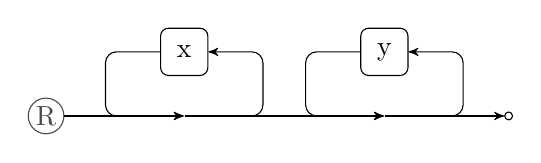
\begin{tikzpicture}
			\node[start] (start) {R};
			\node[junction, right=1 of start] (p1) {};
			\node[junction, right=of p1] (x) {};
			\node[junction, right=1.5 of x] (p2) {};
			\node[junction, right=of p2] (p3) {};
			\node[junction, right=of p3] (y) {};
			\node[junction, right=of y] (p4) {};
			\node[end, right=1 of p4] (end) {};
			\node[box, above=of x] (x1) {x};
			\node[box, above=of y] (y1) {y};

			\graph [use existing nodes] {
				start -> x -> y -> end;
				x ->[vloop] x1 ->[hloop] x;
				y ->[vloop] y1 ->[hloop] y;
			};
		\end{tikzpicture}
		\end{center}

		Og á sama hátt væri endanleg stöðuvél nokkurnveginn svona:

		\begin{center}
			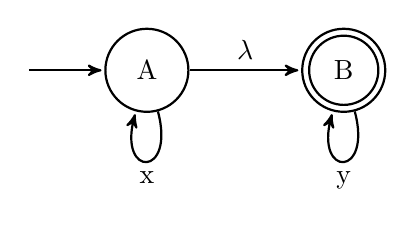
\begin{tikzpicture}[->, >=stealth', shorten >=1pt, auto, node distance=2cm,thick, main node/.style={circle,draw,minimum size=3em}]
				 
				\node[main node] at (1.5,0) (a) {A};
				\node[main node] at (4,0) (b) {B};
				\node[main node, minimum size=2.5em] at (4,0) (bfin) {};


			\path (a) edge node {$\lambda$} (b);
			\path (a) edge [loop below=60] node {x} (a);
			\path (b) edge [loop below=60] node {y} (b);
			\path (0,0) edge node {} (a);

			\end{tikzpicture}
		\end{center}


	\end{document}
